\section{Analysing the system and its architecture}
The architecture of the system is important because it dictates the means by which scalability can be obtained. Fig. \ref{fig:systemArchitecture} presents the architecture of the system we want to extend. The architecture is an extension of the one presented in \cite{IrimieAndPetcu}. The system is composed of 7 components: "FrontEnd", "Scanner", "Converter", "Presenter", "Remediator", a document database and a message queue. The first five components send messages using the queues and are completely decoupled from one another, from each component perspective the system is only compose of itself and one or more message queues. This decoupling provides grate opportunity for replication and scalability.

\begin{figure}[ht]
\centering
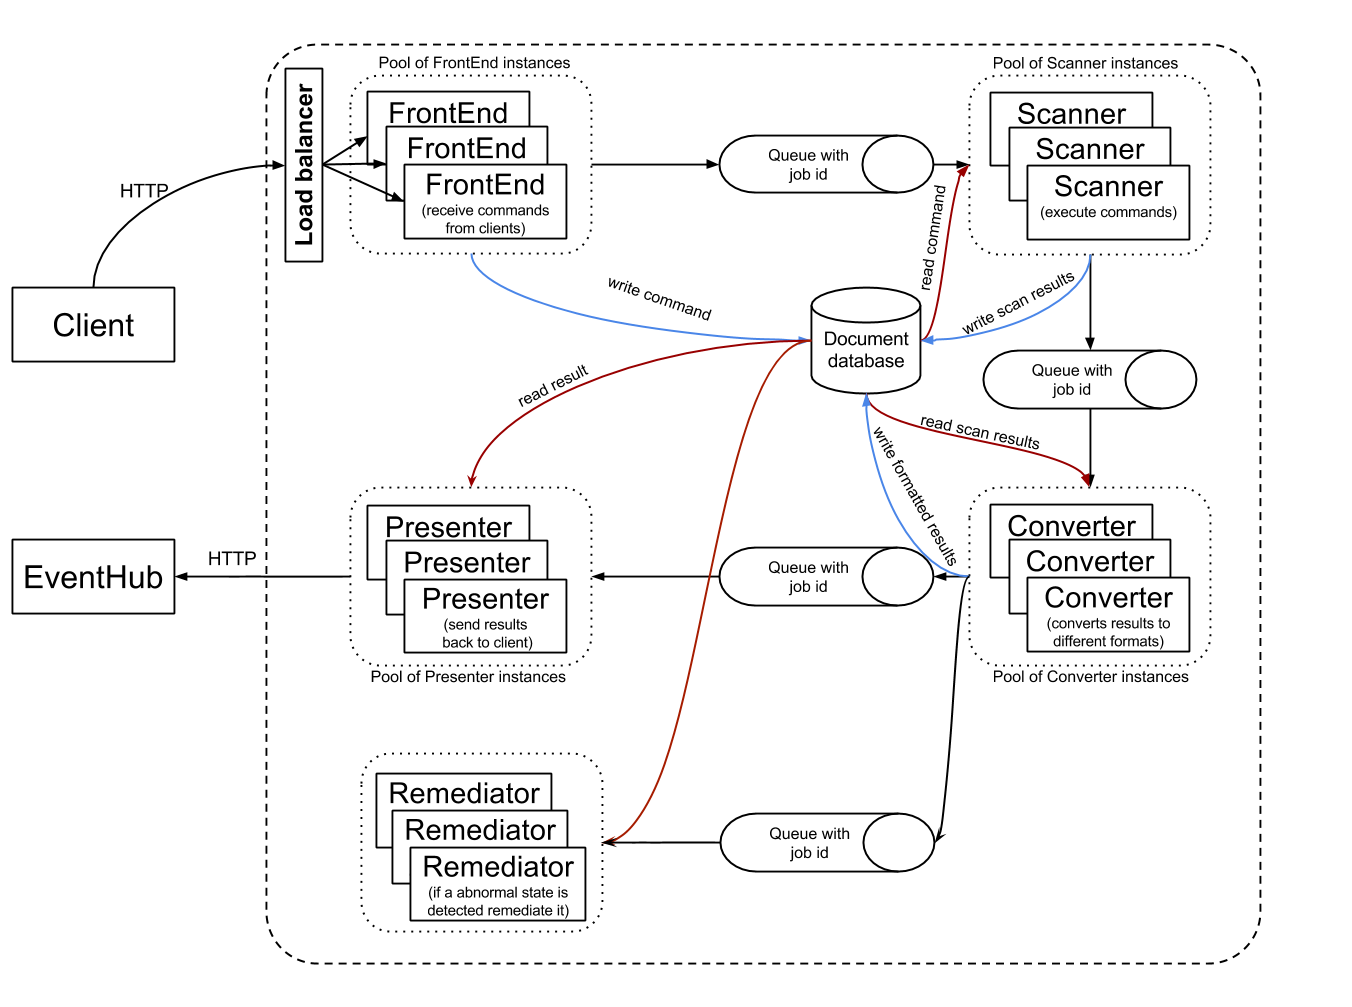
\includegraphics[width=\linewidth]{./img/MonitoringSystemArchitectureRemediation.png}
\caption{Distributed monitoring system architecture}
\label{fig:systemArchitecture}
\end{figure}

